\section{Tipologie principali di densità}

\begin{defn}
    \textbf{Densità uniforme su [a, b]} \\
    Sia data $ X $ con densità $ f(x) $
    \begin{equation*}
        f(x; a, b) = \begin{cases}
            \frac{1}{b-a} & a \leq x \leq b \\
            0   &    \text{altrimenti}
        \end{cases}
    \end{equation*}

    Il \textbf{valore atteso è} $ \dfrac{a + b}{2} $. La \textbf{varianza} è $
    \dfrac{(b - a)^2}{12}$

    \begin{figure}[htbp]
        \centering

        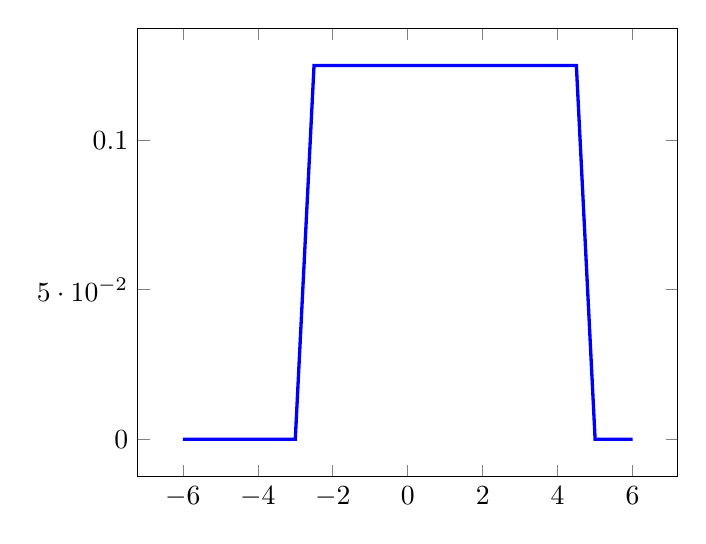
\begin{tikzpicture}[declare function={unipdf(\x,\xl,\xu)=
        (\x>\xl)*(\x<\xu)*1/(\xu-\xl);}]
            \begin{axis}[] \addplot[very thick, blue][domain=-6:6]
                {unipdf(x,-3,5)};
            \end{axis}
        \end{tikzpicture}
        \caption{Densità di probabilità uniforme di parametri $a = -3$ e $b = 5$}
        \label{uniform}
    \end{figure}


    La funzione di ripartizione $F$ è definita come
    \begin{equation*}
        F(x) = \int_{-\infty}^x f(t) dt = \begin{cases}
            0 & x \leq a \\
            \frac{x-a}{b-a} & a < x < b \\
            1 & x \geq b
        \end{cases}
    \end{equation*}
    $ F $ è la funzione di ripartizione in tutti i punti in cui $ f $ è continua
    \begin{equation*}
        f(x) = \frac{dF(x)}{dx}
    \end{equation*}

    \begin{figure}[htbp]
        \centering

        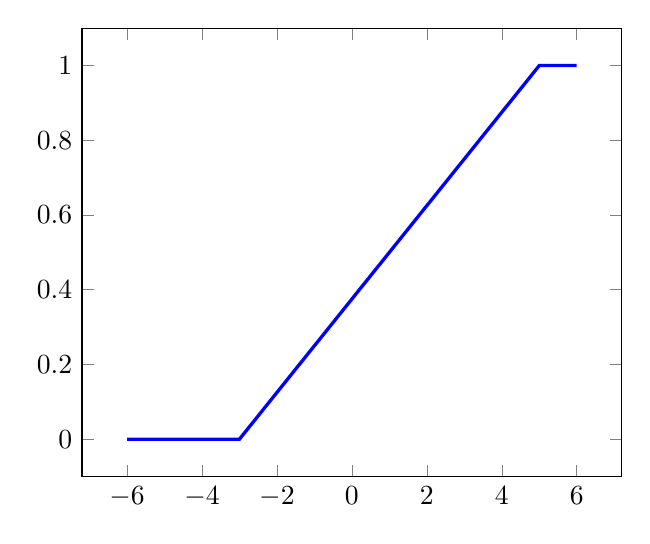
\begin{tikzpicture}[declare function={func(\x,\a,\b) = and(\x > \a, \x <
            \b) * ((\x - \a)/(\b - \a)) + (\x >= \b);}]
            \begin{axis}[] \addplot[very thick, blue][domain=-6:6]
                {func(x,-3,5)};
            \end{axis}
        \end{tikzpicture}
        \caption{Funzione di ripartizione della densità di probabilità uniforme di parametri $a = -3$ e $b = 5$}
        \label{uniformpart}
    \end{figure}

\end{defn}

\begin{defn}
    \textbf{Densità esponenziale di parametro} $ \lambda > 0 $ \\
    Sia data la densità
    \begin{equation*}
        f(x) = \begin{cases}
            \lambda e^{-\lambda x} & x \geq 0 \\
            0 & x < 0
        \end{cases}
    \end{equation*}

    Il valore atteso è $ \dfrac{1}{\lambda} $. La speranza è
    $\dfrac{1}{\lambda^2}$

    \begin{figure}[htbp]
        \centering

        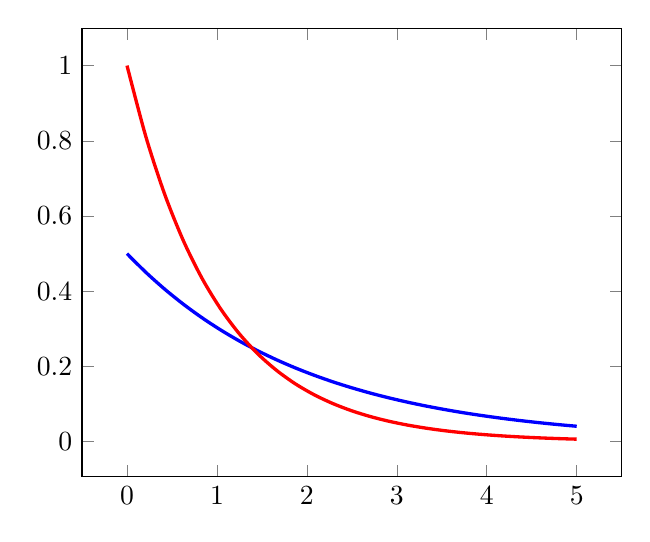
\begin{tikzpicture}[declare function={func(\x,\lambda) =
            (\lambda*e^(-\lambda*\x));}]
            \begin{axis}[smooth] \addplot[very thick, blue][domain=0:5]
                {func(x,0.5)}; \addplot[very thick, red][domain=0:5]
                {func(x,1)};
            \end{axis}
        \end{tikzpicture}
        \caption{Densità di probabilità esponenziale di parametro $\lambda = 0.5$ (blu) e $\lambda = 1$ (rosso)}
        \label{exparam}
    \end{figure}

    \begin{figure}[htbp]
        \centering

        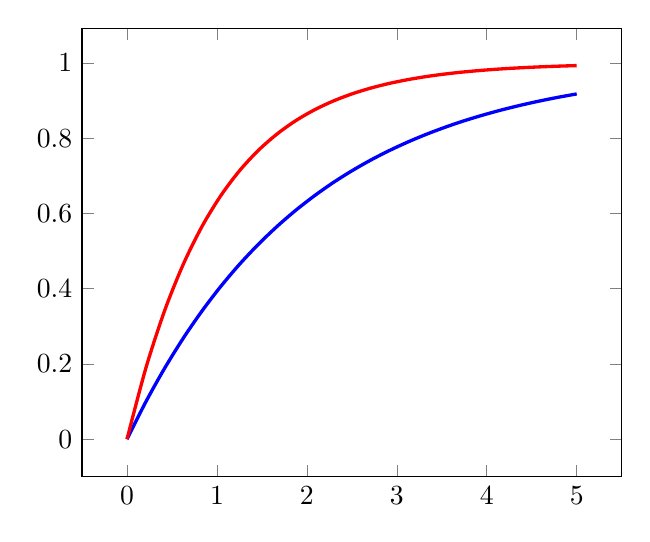
\begin{tikzpicture}[declare function={func(\x,\lambda) = (1 -
            e^(-\lambda*\x));}]
            \begin{axis}[smooth] \addplot[very thick, blue][domain=0:5]
                {func(x,0.5)}; \addplot[very thick, red][domain=0:5]
                {func(x,1)};
            \end{axis}
        \end{tikzpicture}
        \caption{$P(X \leq x)$ (funzione di ripartizione) di un'esponenziale di parametro $\lambda = 0.5$ (blu) e $\lambda = 1$ (rosso)}
        \label{exparam2}
    \end{figure}

    La funzione di ripartizione $ F $ è
    \begin{equation*}
        F(x) = \int_{-\infty}^{x} f(t) dt = \begin{cases}
            0 & x \leq 0 \\
            1 - e^{-\lambda x} & x > 0 \\
        \end{cases}
    \end{equation*}

\end{defn}

% //TODO ???????
\begin{note}
    Se X ha densità

    \begin{equation*}
        \p{X = x} = \int_x f(t) dt = 0
    \end{equation*}
\end{note}

\begin{defn}
    \textbf{Densità di Cauchy} \\
    La densità di Cauchy (detta anche distribuzione di Cauchy o distribuzione di
    Lorentz) è una particolare funzione di densità che descrive nel piano
    euclideo l'intersezione tra l'asse delle ascisse ed una retta passante per
    un punto fissato ed inclinata ad un angolo che segue la distribuzione
    continua uniforme. I momenti di una distribuzione di Cauchy non sono
    definiti.

    \begin{equation*}
        \begin{aligned}
            f(x) = \frac{1}{\pi (1+x)^2}
        \end{aligned}
    \end{equation*}


    \begin{figure}[htbp]
        \centering

        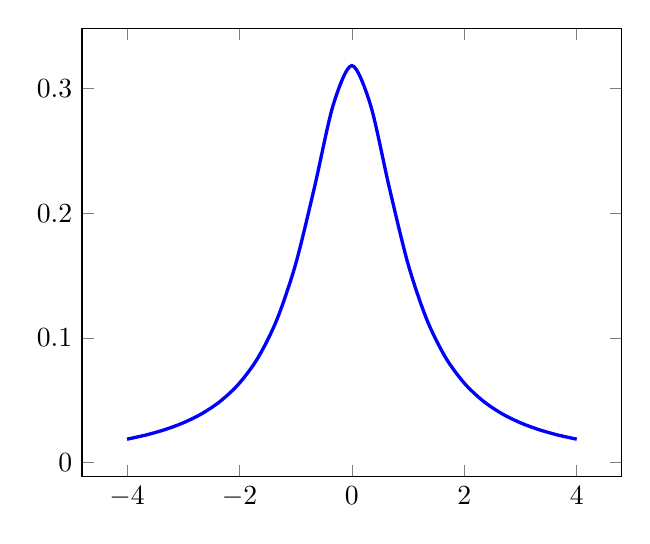
\begin{tikzpicture}[declare function={func(\x) = (1/(pi * (1 +
            \x^2)));}]
            \begin{axis}[smooth] \addplot[very thick, blue][domain=-4:4]
                {func(x)};
            \end{axis}
        \end{tikzpicture}
        \caption{Densità di probabilità di Cauchy}
        \label{cauchy}
    \end{figure}


    \begin{prop}
        La distribuzione di Cauchy è una densità di probabilità.
    \end{prop}

    \begin{proof}
        \begin{equation*}
            \begin{aligned}
                \frac{1}{\pi} \int_{-\infty}^{+\infty} \frac{1}{1 + x^2} dx = \frac{1}{\pi} \lim_{M \to +\infty} \int_{-M}^{M} \frac{dx}{1 + x^2} \\
                = \frac{1}{\pi} \lim_{M \to +\infty} \left( \arctan(M) - \arctan(-M) \right) = \frac{1}{\pi} \left( \frac{\pi}{2} + \frac{\pi}{2} \right) = 1
            \end{aligned}
        \end{equation*}
    \end{proof}

    \begin{prop}
        La densità di Cauchy non ha momenti.
    \end{prop}

    \begin{proof}
        \begin{equation*}
            \begin{aligned}
                \frac{1}{\pi} \int_{-\infty}^{+\infty} \frac{\abs{x}{}}{1 + x^2} dx = \frac{1}{\pi} \int_{0}^{+\infty} \frac{2x}{1 + x^2} dx =
                \frac{1}{\pi} \left[ \log(1 + x^2) \right]_{0}^{+\infty} = - \frac{1}{\pi} \cdot 0 + \frac{1}{\pi} \cdot +\infty = +\infty \\
                \implies \nexists \E{X}
            \end{aligned}
        \end{equation*}
    \end{proof}
\end{defn}

\begin{defn}
    \textbf{Distribuzione normale (Gaussiana)} \\
    La distribuzione Gaussiana ha una funzione di densità a forma di campana. È
    utilizzata per rappresentare variabili aleatorie a valori reali che sono
    prodotte dalla somma di tanti piccoli risultati. Ad esempio, la
    distribuzione normale viene utilizzata per modellare l'altezza della
    popolazione, perché l'altezza può essere il risultato di tanti piccoli
    fattori genetici e ambientali.

    Sia data la densità $f(x;\mu, \sigma^2)$ dove $\mu$ è il parametro che
    rappresenta il valore atteso e $\sigma^2$ rappresenta la varianza. Si indica
    comunemente con $N(\mu, \sigma^2)$. La densità Gaussiana $N(0,1)$ di
    parametri $\mu = 0$ e $\sigma^2 = 1$ viene detta \textbf{densità Gaussiana
    standard}. Dal grafico si nota che la campana si sposta orizzontalmente al
    variare di $\mu$, mentre al variare della varianza $\sigma^2$ la campana
    "cambia forma".

    \begin{equation*}
        \begin{aligned}
            f(x) = \frac{1}{\sigma \sqrt{2\pi}} e^{-\dfrac{(x - \mu)^2}{2 \sigma^2}}
        \end{aligned}
    \end{equation*}

    \pgfmathdeclarefunction{gauss}{2}{%
     \pgfmathparse{1/(#2*sqrt(2*pi))*exp(-((x-#1)^2)/(2*#2^2))}%
    }

    \begin{figure}[htbp!]
        \centering

        \begin{tikzpicture}[]
            \begin{axis}[scale=2, smooth]
                \addplot[very thick, blue][domain=-5:6]{gauss(0, 1.2)};
                \addplot[very thick, red][domain=-5:6]{gauss(0.66, 0.47)};
                \addplot[very thick, green][domain=-5:6]{gauss(1.44, 1.92)};
            \end{axis}
        \end{tikzpicture}
        \caption{Distribuzione di probabilità Gaussiana con parametri $\mu = 0, \sigma^2 = 1.44$ (blu); $\mu = 0.66, \sigma^2 = 0.22$ (rosso); $\mu =1.44, \sigma^2 = 3.68$ (verde)}
        \label{gaussian}
    \end{figure}
\end{defn}

\clearpage

